\chapter{Аналитический раздел}
\label{cha:analysis}

\section{Постановка задачи}

В соответствии с заданием на курсовую работу необходимо разработать загружаемый модуль ядра для ОС Linux, позволяющий скрывать файлы или запрещать их изменение, чтение и удаление. Предусмотреть возможность ввода пароля для отображения файлов или разрешения операций над ними. Предоставить пользователю возможность задавать список таких файлов.

Для достижения поставленной цели необходимо решить следующие задачи:

\begin{itemize}
	\item изучить принцип работы файловой системы Linux;
	\item изучить возможности перехвата функций в ядре Linux;
	\item изучить возможность передачи данных из режима пользователя в режим ядра;
	\item разработать алгоритмы и структуру программного обеспечения;
	\item реализовать программное обеспечение;
	\item протестировать работоспособность разработанного программного обеспечения.
\end{itemize}

\section{Файловая система UNIX}

Файловая система UNIX представляет собой иерархическую древовидную структуру, состоящую из каталогов и файлов. Начинается она с каталога, который называется корнем (root), а имя этого каталога представлено единственным символом --- /.

Каталог представляет собой файл, в котором содержатся каталожные записи. Логически каждую такую запись можно представить в виде структуры, состоящей из имени файла и дополнительной информации, описывающей атрибуты файла. Атрибуты файла --- это такие характеристики, как тип файла (обычный файл или каталог), размер файла, владелец файла, права доступа к файлу (есть ли у других пользователей доступ к файлу), время последней модификации файла \cite{stiven}.

Имена элементов каталога называются именами файлов. Только два символа не могут встречаться в имени файла --- это прямой слэш (/) и нулевой символ (\textbackslash 0). Символ слэша разделяет имена файлов, из которых состоит строка пути к файлу, а нулевой символ обозначает конец этой строки.

Всякий раз, когда создается новый каталог, автоматически создаются два файла: . (называется точка) и .. (называется точка--точка). Под именем <<точка>> подразумевается текущий каталог, а под именем <<точка--точка>> --- родительский. 

Сегодня используются самые разные реализации файловых систем UNIX. Например, Solaris поддерживает несколько типов дисковых файловых систем: традиционную для BSD--систем UNIX File System (UFS), DOS--совместимую файловую систему под названием PCFS и файловую систему, предназначенную для компакт--дисков --- HSFS \cite{stiven}. 

На рисунке \ref{fig:fs} представлен диск, поделенный на несколько разделов. Каждый из разделов может содержать файловую систему. 

\clearpage

\begin{figure}[ph!]
	\center{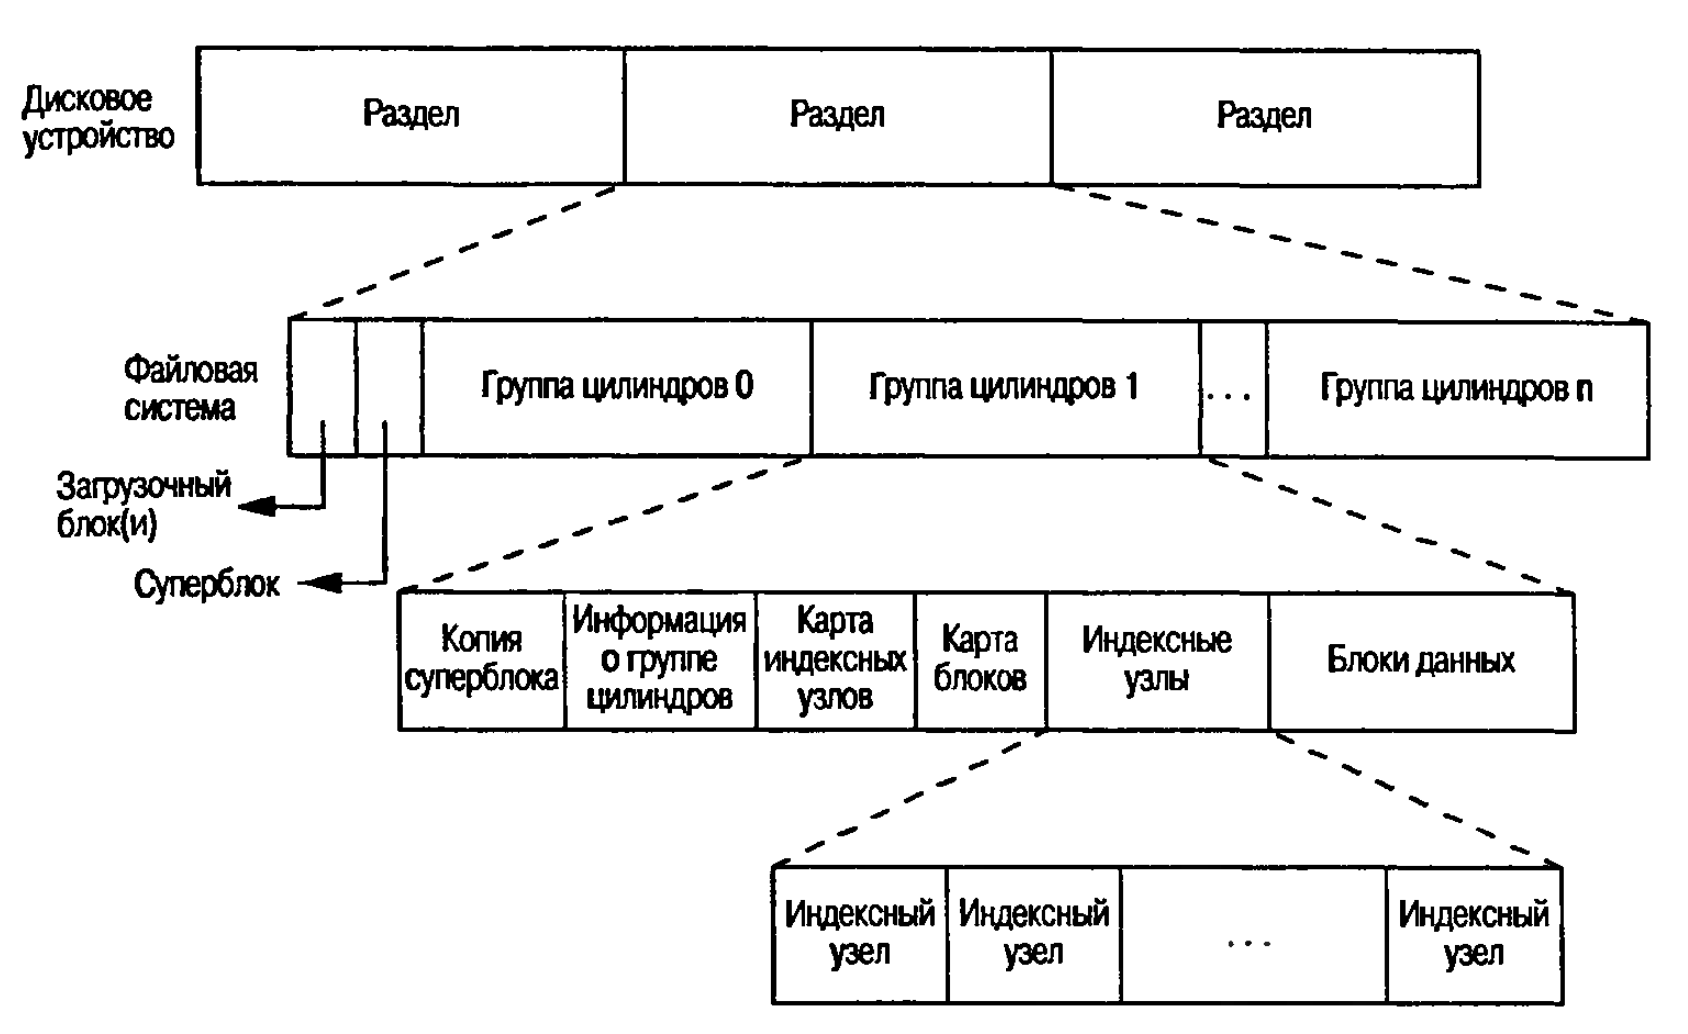
\includegraphics[scale=0.52]{img/fs.png}}
	\caption{Дисковое устройство, разделы и файловая система}
	\label{fig:fs}
\end{figure}

Индексные узлы --- это записи фиксированной длины, которые содержат большую часть сведений о файлах.


\section{Файловый ввод--вывод}

К операциям файлового ввода--вывода относятся открытие файла, чтение из файла, запись в файл и так далее. Большинство операций файлового ввода--вывода в UNIX можно выполнить с помощью пяти функций: open, read, write, lseek и close. 

Все открытые файлы представлены в ядре файловыми дескрипторами. Файловый дескриптор --- это неотрицательное целое число. Когда процесс открывает существующий файл или создает новый, ядро возвращает ему файловый дескриптор. Чтобы выполнить запись в файл или чтение из него, нужно передать функции read или write его файловый дескриптор, полученный в результате вызова функции open или create.

В соответствии с принятыми соглашениями командные оболочки UNIX ассоциируют файловый дескриптор 0 со стандартным устройством ввода процесса, 1 --- со стандартным устройством вывода и 2 --- со стандартным устройством вывода сообщений об ошибках. Это соглашение используется командными оболочками и большинством приложений, но не является особенностью ядpa UNIX. Тем не менее многие приложения не смогли бы работать, если это соглашение было бы нарушено.

\subsection{Функция open}

Системный вызов open() открывает файл, указанный в pathname. Если указанный файл не существует, он может (если указан флаг O\_CREATE) быть создан open().

\begin{lstlisting}[label=code:open,caption=Функция open]
#include <fcntl.h>

int open (const char *pathname, int flags);
int open (const char *pathname, int flags, mode_t mode);
\end{lstlisting}

Возвращаемое значение open() --- дескриптор файла, неотрицательное целое число, которое используется в последующих системных вызовах для работы с файлом.

Параметр flags --- это флаги, которые собираются с помощью побитовой операции ИЛИ из таких значений, как:

\textit{O\_EXEC} — открыть только для выполнения (результат не определен, при открытии директории).

\textit{O\_RDONLY} — открыть только на чтение.

\textit{O\_RDWR} — открыть на чтение и запись.

\textit{O\_SEARCH} — открыть директорию только для поиска (результат не определен, при использовании с файлами, не являющимися директорией).

\textit{O\_WRONLY} — открыть только на запись.

\textit{O\_APPEND} — файл открывается в режиме добавления, перед каждой операцией записи файловый указатель будет устанавливаться в конец файла.

\textit{O\_CLOEXEC} — устанавливает флаг close-on-exec для нового файлового дескриптора, указание этого флага позволяет программе избегать дополнительных операций fcntl \textit{F\_SETFD} для установки флага \textit{FD\_CLOEXEC}.

\textit{O\_CREAT} — если файл не существует, то он будет создан.

\textit{O\_DIRECTORY} — если файл не является каталогом, то open вернёт ошибку.

\textit{O\_DSYNC} — файл открывается в режиме синхронного ввода-вывода (все операции записи для соответствующего дескриптора файла блокируют вызывающий процесс до тех пор, пока данные не будут физически записаны).

\textit{O\_EXCL} — если используется совместно с \textit{O\_CREAT}, то при наличии уже созданного файла вызов завершится ошибкой.

\textit{O\_NOCTTY} — если файл указывает на терминальное устройство, то оно не станет терминалом управления процесса, даже при его отсутствии.

\textit{O\_NOFOLLOW} — если файл является символической ссылкой, то open вернёт ошибку.

\textit{O\_NONBLOCK} — файл открывается, по возможности, в режиме non-blocking, то есть никакие последующие операции над дескриптором файла не заставляют в дальнейшем вызывающий процесс ждать.

\textit{O\_RSYNC} — операции записи должны выполняться на том же уровне, что и \textit{O\_SYNC}.

\textit{O\_SYNC} — файл открывается в режиме синхронного ввода-вывода (все операции записи для соответствующего дескриптора файла блокируют вызывающий процесс до тех пор, пока данные не будут физически записаны).

\textit{O\_TRUNC} — если файл уже существует, он является обычным файлом и заданный режим позволяет записывать в этот файл, то его длина будет урезана до нуля.

\textit{O\_LARGEFILE} — позволяет открывать файлы, размер которых не может быть представлен типом off\_t (long). Для установки должен быть указан макрос \_LARGEFILE64\_SOURCE

\textit{O\_TMPFILE} — при наличии данного флага создаётся неименованный временный файл.

\textit{O\_PATH} — получить файловый дескриптор, который можно использовать для двух целей: для указания положения в дереве файловой системы и для выполнения операций, работающих исключительно на уровне файловых дескрипторов. Если \textit{O\_PATH} указан, то биты флагов,  отличные от \textit{O\_CLOEXEC}, \textit{O\_DIRECTORY} и \textit{O\_NOFOLLOW}, игнорируются.


Третий параметр mode всегда должен быть указан при использовании 

\noindent\textit{O\_CREAT}; во всех остальных случаях этот параметр игнорируется.


Схема алгоритма работы системного вызова ореn() представлена на рисунке \ref{fig:open}.
\clearpage
\begin{figure}[ph!]
	\center{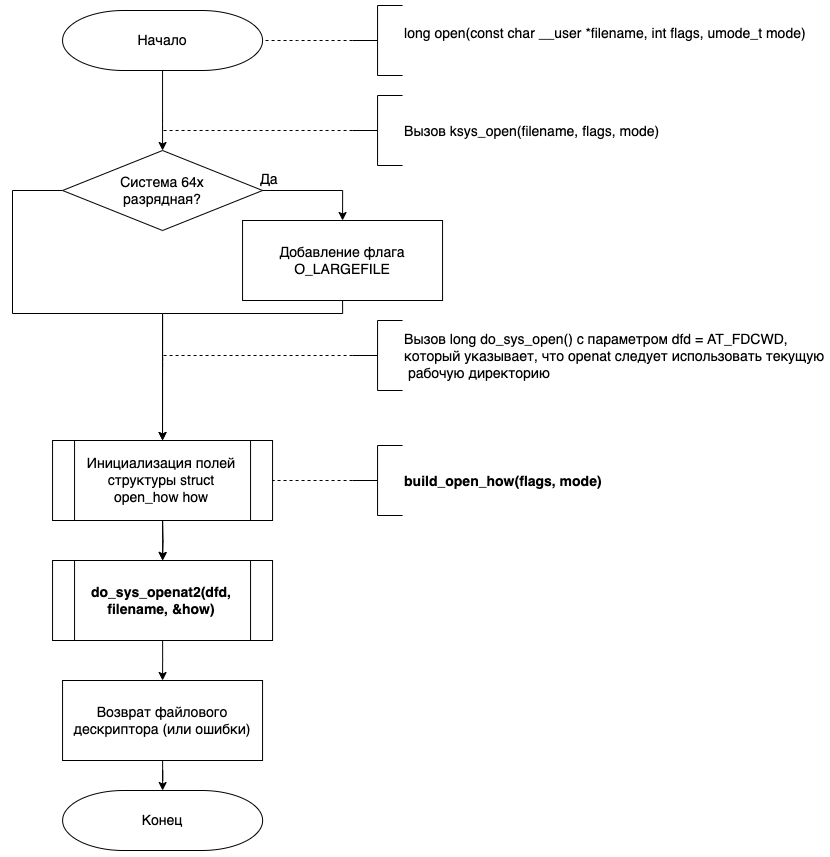
\includegraphics[scale=0.49]{img/open.png}}
	\caption{Схема алгоритма работы системного вызова ореn()}
	\label{fig:open}
\end{figure}

Функция open гарантирует, что возвращаемый ею дескриптор файла будет представлять собой наименьшее не используемое в качестве дескриптора положительное число.



\subsection{Функция write}

Запись данных в открытый файл производится функцией write.

\begin{lstlisting}[label=code:write,caption=Функция write]
#include <unistd.h>
	
ssize_t write(int fd, const void *buf, size_t size);
\end{lstlisting}

Возвращаемое значение обычно совпадает со значением аргумента size, в противном случае возвращается признак ошибки. Наиболее распространенные случаи, когда возникает ошибка записи, --- это переполнение диска или превышение ограничения на размер файла для заданного процесса.

Для обычных файлов запись начинается с текущей позиции файла. Если при открытии файла был указан флаг O\_APPEND, текущая позиция устанавливается в конец файла перед началом каждой операции записи. По окончании записи значение текущей позиции увеличивается на количество фактически записанных байт.


\subsection{Функции link, unlink}

На индексный узел любого файла могут указывать несколько каталожных записей. Такие ссылки создаются с помощью функции link.

\begin{lstlisting}[label=code:link,caption=Функция link]
#include <unistd.h>

int link(const char *existingpath, const char *newpath);
\end{lstlisting}

Эта функция создает в каталоге новую запись с именем newpath, которая будет указывать на существующий файл existingpath. Если запись с именем newpath уже существует, функция вернет признак ошибки. Создается только последний компонент полного пути newpath, все промежуточные компоненты должны существовать к моменту вызова функции.

Операции создания новой записи в каталоге и увеличения счетчика ссылок должны выполняться атомарно. 

Большинство реализаций требуют, чтобы оба пути находились в пределах одной файловой системы, хотя стандарт POSIX.1 допускает возможность создания ссылок на файлы, расположенные в других файловых системах. Если поддерживается создание жестких ссылок на каталоги, то эта операция может выполняться только суперпользователем. Причина такого ограничения состоит в том ,что создание жесткой ссылки на каталог может привести к появлению замкнутых <<петель>> в файловой системе, и большинство обслуживающих ее утилит не смогут обработать их надлежащим образом. По этой же причине многие реализации файловых систем вообще не допускают создания жестких ссылок на каталоги.

Удаление записей из каталога производится с помощью функции unlink.

\begin{lstlisting}[label=code:unlink,caption=Функция unlink]
#include <unistd.h>

int unlink(const char *pathname);
\end{lstlisting}

Эта функция удаляет запись из файла каталога и уменьшает значение счетчика ссылок на файл pathname. Если на файл указывает несколько ссылок, то его содержимое будет через них по--прежнему доступно. В случае ошибки файл не изменяется.


\subsection{Функция getdents}

Функция getdents возвращает записи каталога.

\begin{lstlisting}[label=code:getdents,caption=Функция getdents]
#include <unistd.h>
	
int getdents(unsigned int fd, struct linux_dirent *dirp, unsigned int count);
\end{lstlisting}

Системный вызов getdents() читает несколько структур linux\_dirent из каталога, на который указывает открытый файловый дескриптор fd, в буфер, указанный в dirp. В аргументе count задаётся размер этого буфера.

Структура linux\_dirent определена следующим образом \cite{linux}:
\begin{lstlisting}[label=code:linuxdirent,caption=Структура linux\_dirent]
struct linux_dirent {
	unsigned long	d_ino;
	unsigned long	d_off;
	unsigned short	d_reclen;
	char	d_name[1];
};
\end{lstlisting}

В d\_ino указан номер inode. В d\_off задается расстояние от начала каталога до начала следующей linux\_dirent. В d\_reclen указывается размер данного linux\_dirent целиком. В d\_name задается имя файла, завершающееся null.
d\_type --- тип файла.
В нем содержится одно из следующих значений (определённых в <dirent.h>):
\begin{itemize}
	\item DT\_BLK (блочное устройство);
	\item DT\_CHR (символьное устройство);
	\item DT\_DIR (каталог);
	\item DT\_FIFO (именованный канал (FIFO));
	\item DT\_LNK (символическая ссылка);
	\item DT\_REG (обычный файл);
	\item DT\_SOCK (доменный сокет UNIX);
	\item DT\_UNKNOWN (неизвестный тип).
\end{itemize}


Первоначальный системный вызов Linux getdents() не работал с файловыми системами большого размера и большими смещениями файлов. В связи с этим, в Linux 2.4 была добавлен getdents64().

Системный вызов getdents64() подобен getdents(), за исключением того, что второй аргумент является указателем на буфер, содержащий структуры следующего типа:

\begin{lstlisting}[label=code:linuxdirent64,caption=Структура linux\_dirent64]
struct linux_dirent64 {
	ino64_t		d_ino;
	off64_t		d_off;    
	unsigned short	d_reclen; 
	unsigned char	d_type;  
	char	d_name[]; 
};
\end{lstlisting}


\section{Перехват функций в ядре с помощью ftrace}

Название ftrace представляет собой сокращение от Function Trace~---~трассировка функций. Однако возможности этого инструмента гораздо шире: с его помощью можно отслеживать контекстные переключения, измерять время обработки прерываний, высчитывать время на активизацию заданий с высоким приоритетом и многое другое \cite{ftrace}.

Ftrace был разработан Стивеном Ростедтом и добавлен в ядро в 2008 году, начиная с версии 2.6.27. Ftrace --- фреймворк, предоставляющий отладочный кольцевой буфер для записи данных. Собирают эти данные встроенные в ядро программы--трассировщики \cite{ftrace}.

Работает ftrace на базе файловой системы debugfs, которая в большинстве современных дистрибутивов Linux смонтирована по умолчанию. 

Каждую перехватываемую функцию можно описать следующей структурой:
\clearpage
\begin{lstlisting}[label=code:ftracehook,caption=Структура ftrace\_hook]
struct ftrace_hook {
	const char *name;
	void *function;
	void *original;
	
	unsigned long address;
	struct ftrace_ops ops;
};
\end{lstlisting}

Поля структуры:

\textit{name} --- имя перехватываемой функции;

\textit{function} ---  адрес функции--обертки, которая будет вызываться вместо перехваченной функции;

\textit{original} ---  указатель на место, куда следует записать адрес перехватываемой функции, заполняется при установке;

\textit{address} --- адрес перехватываемой функции, заполняется при установке;

\textit{ops} --- служебная информация ftrace.

Пользователю необходимо заполнить только первые три поля: name, function, original. 

\begin{lstlisting}[label=code:ftracehookexm,caption=Пример заполнения структуры ftrace\_hook]
#define HOOK(_name, _function, _original)       \
{                                       \
	.name = (_name),                    \
	.function = (_function),            \
	.original = (_original),            \
}

static struct ftrace_hook hooked_functions[] = {
	HOOK("sys_clone",   fh_sys_clone,   &real_sys_clone),
	HOOK("sys_execve",  fh_sys_execve,  &real_sys_execve),
};
\end{lstlisting}



\section*{Вывод}

В результате проведенного анализа был определен способ перехвата системных вызовов в ядре --- путем регистрации функций перехвата с использованием ftrace. Были определены функции, которые необходимо перехватить.